% !TEX encoding = UTF-8
% !TEX TS-program = pdflatex
% !TEX root = ../relazione-finale.tex

%**************************************************************
\chapter{Introduzione}
\label{cap:introduzione}
%**************************************************************

\intro{Nelle sezioni di questo capitolo parlerò dell'idea alla base dello svolgimento dello stage e dei rischi derivati dalle scelte effettuate.}\\

% \noindent Esempio di utilizzo di un termine nel glossario \\
% \gls{api}. \\
%
% \noindent Esempio di citazione in linea \\
% \cite{site:agile-manifesto}. \\
%
% \noindent Esempio di citazione nel pie' di pagina \\
% citazione\footcite{womak:lean-thinking} \\

%**************************************************************
\section{L'idea}

Internet Of Things è un paradigma tecnologico diffusosi nell'ultimo decennio. Questa locuzione fa riferimento a un insieme di oggetti,
di varia natura e utilizzo, che interagiscono tra loro e che permettono all'utente di interagire con essi.
L'idea che mi ha spinto allo sviluppo e alla realizzazione del progetto di stage è stata quella unificare in un unico centro di controllo
tutti gli eventuali dispositivi connessi alla rete domestica dell'utente, permettendo
tuttavia allo stesso di accedere all'interfaccia proprietaria di ciascun dispositivo.
L'obiettivo di una tale dashboard non è quindi \textit{intrappolare} l'utente in un unico ecosistema domotico,
bensì quello di facilitare la consultazione delle informazioni più frequentemente richieste dall'utente provenienti da più ecosistemi distinti.

Per assicurare prestazioni, affidabilità (\textit{availability}) e scalabilità del prodotto sviluppato e per aggiungere una natura formativa al progetto di stage,
ho scelto di progettare il prodotto secondo l'architettura a microservizi.

\subsection{IoT}
\label{intro-iot}
L'idea di una rete di dispositivi smart fu presa in considerazione fin dal 1982, quando un distributore automatico di bibite dell'Università di Carnegie Mellon venne opportunamente modificato per accedere al suo inventario di bibite. Quel distributore automatico divenne il primo apparecchio collegato ad Internet.
\footcite{site:mellon-uni}

Nel corso degli anni '90 il mondo accademico e il mondo dell'industra legata alla produzione continuarono a sperimentare evolvendo il \textit{concept} iniziale, arrivando alla conclusione che l'\textit{Ubiquitous Computing} non si debba riferire solamente ai \textit{computer}, ma debba espandersi agli oggetti di utilizzo quotidiano. Questa visione dovette scontrarsi con i limiti della microelettronica di allora: la produzione di semiconduttori non era ancora pronta a supportare la potenziale domanda e i costi per sostenere l'ampliamento degli impianti non erano facilmente assorbibili in breve tempo.
\footcite{site:mit-weiser}

Il termine \textit{"Internet of Things"} fu coniato da Kevin Ashton nel 1999.
\footcite{site:iot-kashton}
L'origine dell'espressione, riassumendo le parole dell'autore, deriva dal fatto che la maggior parte delle informazioni presenti su Internet sono state e sono inserite da utenti "umani", soggetti quindi a concentrazione, precisione e tempo limitate;
se queste informazioni fossero invece inserite da macchine senza l'aiuto di un utente umano, la maggior qualità delle stesse garantirebbe
\begin{itemize}
  \item maggiore capacità di tracciamento delle risorse;
  \item minor spreco di risorse;
  \item minor costo per la gestione delle risorse.
\end{itemize} % mantenere almeno 2 righe sotto


Grazie agli avanzamenti nei processi di produzione dei semiconduttori, dovuti alla crescita dei mercati del consumo di massa, allo sviluppo di un numero sempre maggiore di tecnologie volte a migliorare l'efficienza e l'affidabilità dei circuiti integrati e alla sempre maggior diffusione di tecnologie per la trasmissione di informazioni senza fili, dai primi anni 2000 il concetto alla base dell'IoT è stato sviluppato da un numero sempre maggiore di aziende negli ambiti più disparati (\textit{home automation}, \textit{manufacturing}, \textit{smart agriculture}, etc.).
\footcite{site:pc-to-things}

Con Internet of Things si intende una rete di dispositivi interconnessi, individuabili in modo univoco e che possono comunicare informazioni.
I dispositivi presenti in una rete possono comunicare con due tipologie di attori diverse:
\begin{itemize}
  \item se la comunicazione avviene con altri dispositivi si parla di comunicazione M2M (\textit{Machine to Machine}, ovvero comunicazione tra macchine);
  \item se la comunicazione avviene interagendo con il mondo reale si parla di comunicazione M2H (\textit{Machine to Human}, ovvero comunicazione tra macchina e utente).
\end{itemize}


Il termine "Things" nel contesto IoT si riferisce a una varietà di dispositivi come ad esempio: videocamere di sorveglianza, automobili a guida autonoma e assistita oppure piccoli e grandi elettrodomestici casalinghi. Questi dispositivi, soprannominati anche \textit{smart object}, raccolgono informazioni utili in base agli attori con cui comunicano:
\begin{itemize}
  \item se i dispositivi comunicano in modo M2M, le informazioni vengono impiegate al supporto di tecnologie esistenti, integrandosi nel flusso di informazioni esistente;
  \item se i dispositivi comunicano in modo M2H, le informazioni vengono in aiuto delle persone che interagiscono con essi.
\end{itemize}


L'interesse verso il tema IoT è cresciuto esponenzialmente sia nel mercato consumer che in quello enterprise e secondo Forbes (\footcite{site:forbes-iot}) diventerà nel prossimo quinquennio uno dei settori dell'ITC più redditizi.
É interessante osservare anche la popolarità dei termini di ricerca correlati all'IoT: i dati sono stati ottenuti interrogando il servizio \url{https://trends.google.com/trends}, il quale consente di effettuare analisi sulla popolarità delle stringhe di ricerca immesse nel motore di ricerca di Google.
Ciascun grafico a linea (\textit{line chart} in inglese) presenta nelle ordinate il grado di popolarità della \textit{query} di ricerca, valutato da 0 (popolarità minima) a 100 (popolarità massima), e nelle ascisse l'arco temporale in analisi.

\begin{figure}[!ht]
    \centering
    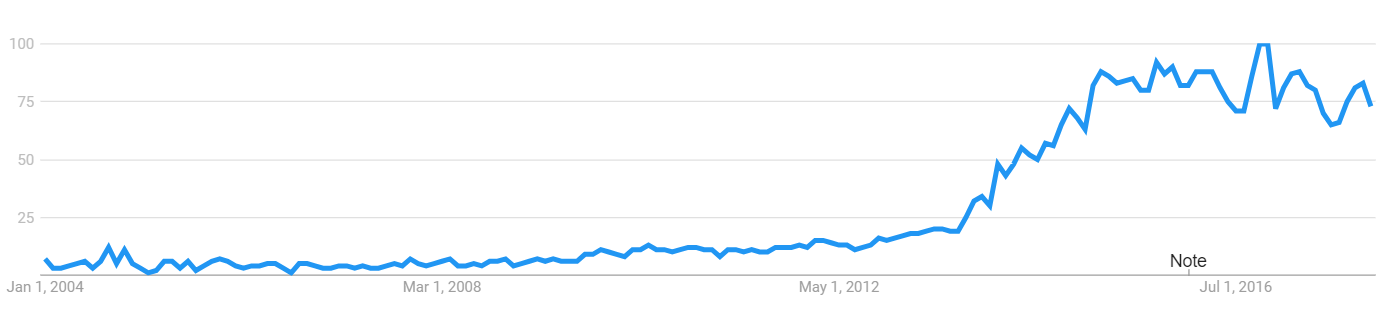
\includegraphics[width=0.9\columnwidth]{intro/internet-of-things-query-interest-worldwide}
    \caption{Andamento dell'interesse per la stringa di ricerca \textit{"internet of things"}. \\ \cite{site:iot-long-trend}}
    \label{fig:internet-of-things-query-interest}
\end{figure}

\begin{figure}[!ht]
    \centering
    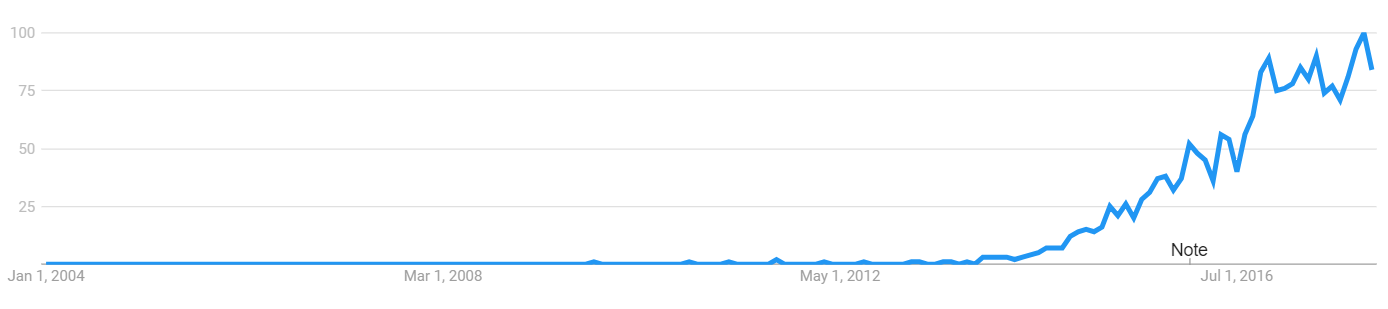
\includegraphics[width=0.9\columnwidth]{intro/iot-devices-query-interest-worldwide}
    \caption{Andamento dell'interesse per la stringa di ricerca \textit{"iot devices"}. \\ \cite{site:iot-devices-trend}}
    \label{fig:iot-devices-query-interest}
\end{figure}

\begin{figure}[!ht]
    \centering
    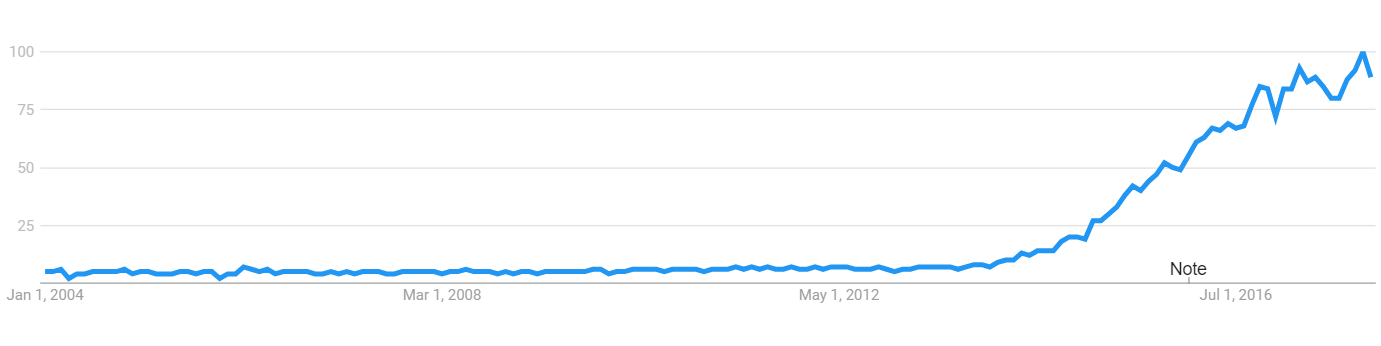
\includegraphics[width=0.9\columnwidth]{intro/iot-query-interest-worldwide}
    \caption{Andamento dell'interesse per la stringa di ricerca \textit{"iot"}. \\ \cite{site:iot-short-trend}}
    \label{fig:iot-query-interest}
\end{figure}

Sintetizzando le previsioni di Forbes con l'andamento dei termini di ricerca legati all'IoT, visibili alle figure ~\ref{fig:internet-of-things-query-interest}, ~\ref{fig:iot-devices-query-interest} e ~\ref{fig:iot-query-interest}, si può notare come l'interesse verso l'argomento IoT stia generalmente aumentando o nel caso peggiore resti stabile con l'interesse degli anni precedenti.

\subsection{Architettura a microservizi}

L'espressione \textbf{Architettura a microservizi} è sempre più comune tra gli sviluppatori di applicazioni \textit{enterprise} per descrivere un metodo di progettazione delle applicazioni come insiemi di servizi eseguibili indipendentemente (ogni servizio esegue su un processo indipendente), che comunicano tra loro grazie a meccanismi di comunicazione "leggeri" (solitamente attraverso \gls{api} HTTP).

\paragraph{Caratteristiche delle architetture monolitiche}

Un'applicazione monolitica è progettata e costruita per essere una singola unità in esecuzione. Solitamente un'applicazione web monolitica è divisa in 3 parti:
\begin{itemize}
  \item interfaccia utente (pagine web);
  \item database;
  \item applicazione server.
\end{itemize}


A sua volta, l'applicazione server:
\begin{itemize}
  \item gestisce le richieste HTTP;
  \item esegue la business logic dell'applicazione;
  \item carica e aggiorna dati dal/nel database;
  \item seleziona e popola le pagine web inviate al browser dell'utente.
\end{itemize}


Nelle applicazioni monolitiche la modularità del sistema si ottiene sfruttando i costrutti fondamentali dei linguaggi di programmazione:
\begin{itemize}
  \item funzioni;
  \item classi;
  \item namespace o package.
\end{itemize}


Per aumentare la disponibilità delle applicazioni monolitiche si usa replicare istanze dell'applicazione in molteplici server, bilanciando il traffico verso le applicazioni per mezzo di un \gls{load balancerg}.
Tra i difetti delle applicazioni monolitiche si possono evidenziare:
\begin{itemize}
  \item modifiche a una piccola parte all'applicazione richiedono la ricompilazione e la ridistribuzione dell'applicazione;
  \item all'accrescere della complessità dell'applicazione aumenta anche la difficoltà nel mantenere le modifiche isolate ai moduli di competenza;
  \item scalare l'applicazione richiede l'esecuzione di istanze multiple della stessa applicazione, ignorando di fatto eventuali requisiti di efficienza (solitamente alcune componenti del sistema non richiedono un aumento di throughput).
\end{itemize}

\paragraph{Caratteristiche delle architetture a microservizi}

Per lo stile architetturale a microservizi non esistono definizioni formali, tuttavia è possibile dedurre le caratteristiche che hanno accomunato i progetti diventati nel tempo esempi di best-practice.
Non tutte le architetture a microservizi hanno tutte le caratteristiche elencate in seguito, ma ci si aspetta che la maggior parte delle architetture esibisca quante più caratteristiche possibili.

L'aspetto cruciale delle architetture a microservizi verte sulla definizione di componente: la definizione comunemente accettata è quella di "unità di software che è indipendentemente aggiornabile e sostituibile in un sistema".
Le architetture a microservizi usano i servizi per realizzare tale definizione di componente. A titolo di confronto con gli approcci di sviluppo tradizionali è possibile introdurre la nozione di libreria.
Le librerie sono componenti insiti in un'applicazione tanto da risiedere nello stesso spazio di memoria dell'applicazione e che per essere invocate richiedono una chiamata di funzione in memoria.
I servizi sono componenti che vivono nel sistema come processi separati, sfruttando vari tipi di comunicazione interprocesso: richieste web, chiamate di funzione remote (RPC).

Il vantaggio principale dei servizi rispetto alle librerie consiste nel fatto che i servizi sono rilasciabili indipendentemente dal sistema.
Data la natura dell'architettura a microservizi, modifiche a un singolo servizio comportano il rilascio di una nuova versione solamente per quel servizio e non dell'intera applicazione.
Una buona architettura a microservizi quindi mira a progettare e implementare servizi che circoscrivano chiaramente il loro scopo.

L'uso di servizi come componenti consente inoltre di rendere esplicita l'interfaccia dei componenti.
Spesso solamente la documentazione e la disciplina prevengono usi impropri di una componente da parte di uno sviluppatore esterno, rischiando di causare un alto accoppiamento tra componenti.
I servizi facilitano il rispetto delle interfacce pubblicate attraverso l'uso di meccanismi di chiamate remote esplicite.

Il difetto che si annovera all'uso di servizi come componenti risiede nell'utilizzo di chiamate remote per la comunicazione tra servizi:
esse richiedono più risorse rispetto alle chiamate di funzione intraprocesso e quindi è necessario progettare le API di ciascun servizio rivolgendo maggiore attenzione all'aspetto prestazionale delle stesse.

Altre differenze sono riscontrabili dal punto di vista della suddivisione delle persone impegnate nello sviluppo dell'applicazione.
Solitamente applicazioni complesse sviluppate seguendo l'architettura monolitica sono divise in team con competenze isolate, illustrata graficamente in figura ~\ref{fig:business-organization}:
\begin{itemize}
  \item team esperto in UI;
  \item team specializzato in DB Management;
  \item uno o più team specializzate a realizzare la logica di business.
\end{itemize}


Quando le persone sono così fortemente isolate, anche una semplice modifica può richiedere l'intervento di altre persone in team diversi, causando inefficienze nel processo di sviluppo.

\begin{figure}[H]
  \centering
  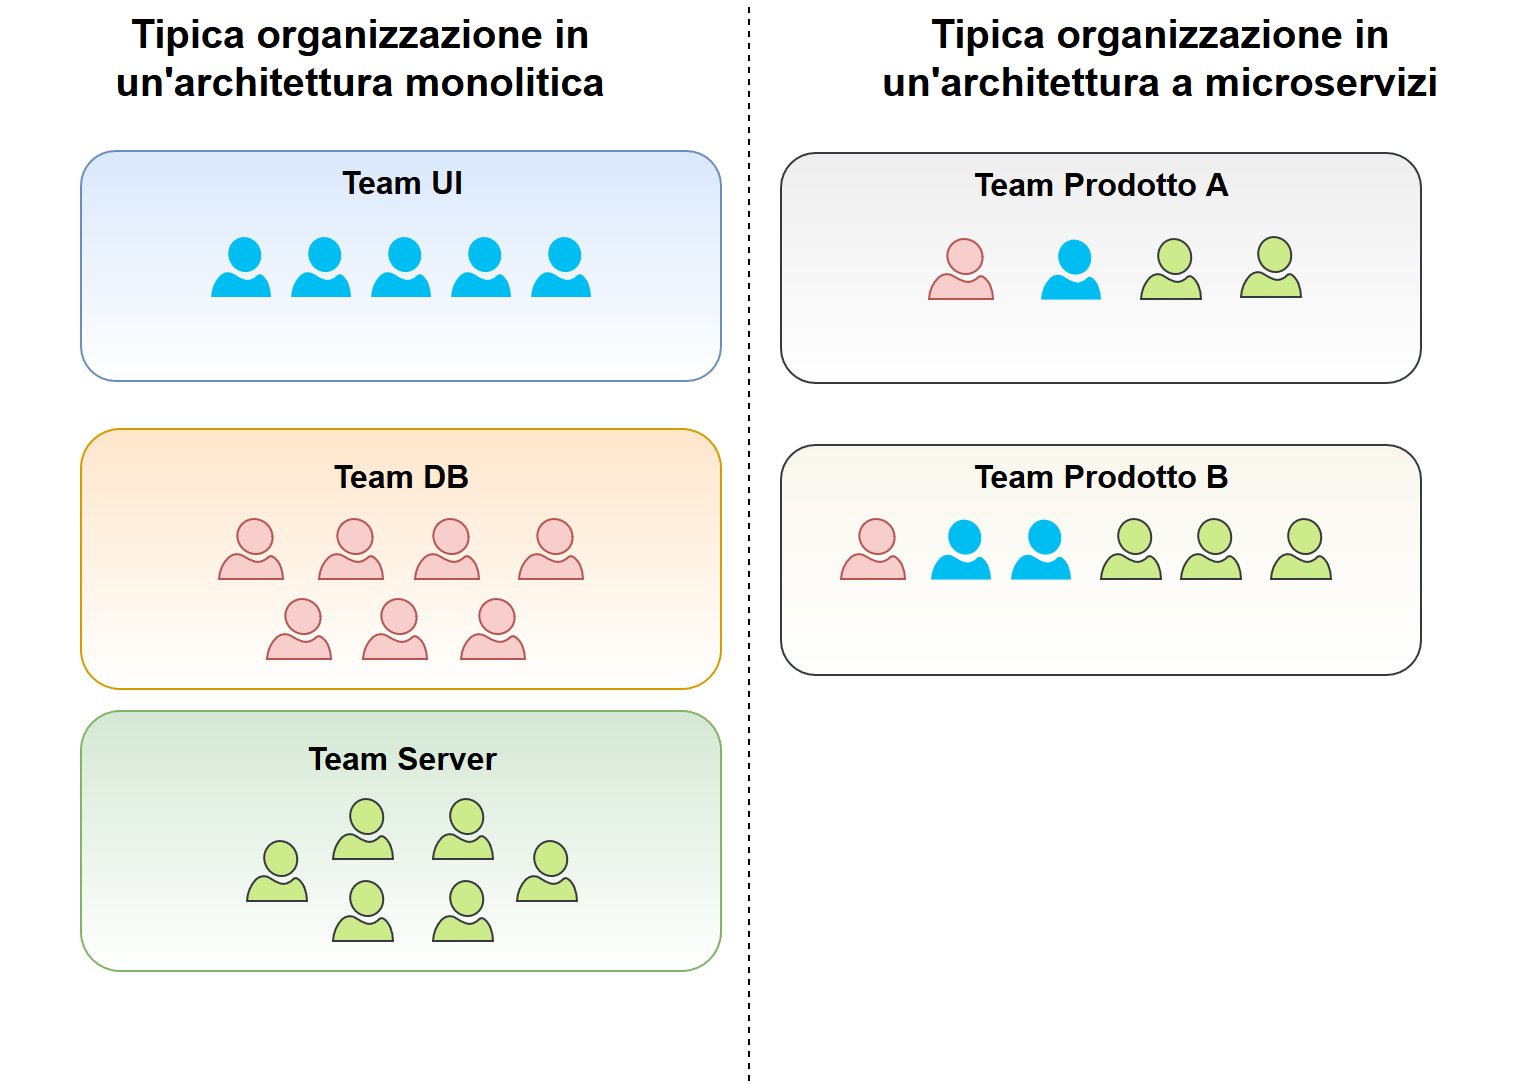
\includegraphics[width=0.9\columnwidth]{intro/business-organization}
  \caption{Illustrazione che mostra la differente organizzazione aziendale in un ambiente di sviluppo monolitico e in un ambiente di sviluppo a microservizi.}
  \label{fig:business-organization}
\end{figure}

L'approccio microservices-oriented alla suddivisione dell'applicazione invece pone l'accento sulle capacità di business: ogni team inerente un particolare settore di business si occupa dell'intero prodotto per quel settore (sviluppando interamente UI, DB, ecc.).
I team in questo approccio sono multidisciplinari e gli scambi con altri settori riflettono le effettive dipendenze tra un settore e un altro all'interno dell'azienda.

Un esempio di quest'approccio alla suddivisione lo si ritrova in Amazon, dove vige il motto "you build, you run it" ("tu lo costruisci, tu lo esegui").
In Amazon ogni team ha completa responsabilità del prodotto anche in ambiente di produzione, mettendo in comunicazione diretta sviluppatori e utenti del prodotto per le attività di supporto e manutenzione.

Applicazioni assemblate con microservizi mirano ad essere più disaccoppiate e più coese possibile: ricevendo una richiesta, applicando la propria logica e producendo una risposta.
Un diagramma esemplificativo di questo concetto lo si trova in figura ~\ref{fig:services-comms}.

\begin{figure}[!ht]
    \centering
    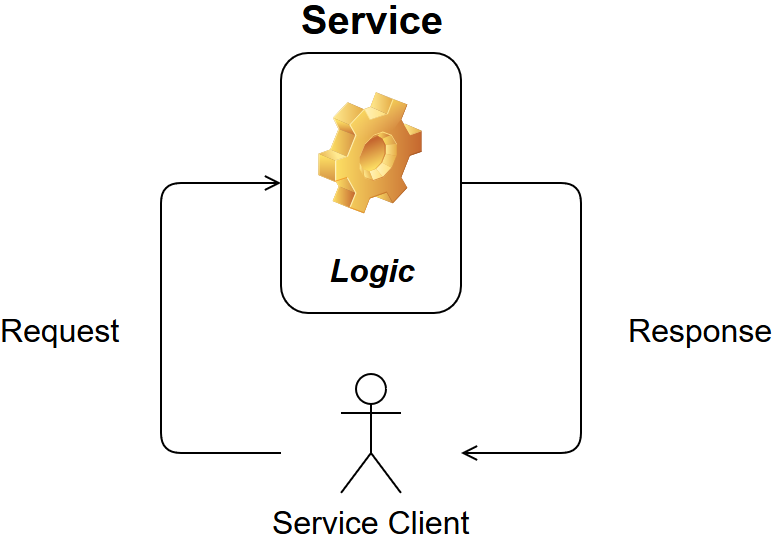
\includegraphics[width=0.9\columnwidth]{intro/services-comms}
    \caption{Illustrazione che mostra come un utente (inteso sia come umano, sia come altro servizio) di un servizio interagisca con esso.}
    \label{fig:services-comms}
\end{figure}

Le comunicazioni tra servizi sono orchestrate usando semplici protocolli REST-like. I due protocolli più usati sono:
\begin{itemize}
  \item richieste/risposte HTTP secondo API ben dettagliate;
  \item messaggistica in un canale di comunicazione snello. I servizi producono e consumano i messaggi che circolano nel canale di comunicazione, secondo regole di accesso definite.
\end{itemize}


Quando un'applicazione è suddivisa in molteplici componenti sorgono naturalmente dubbi sulla gestione delle informazioni che ciascuna componente gestisce.
Solitamente nelle architetture monolitiche i domini dell'applicazione vengono astratti scegliendo una fra le tecniche di modellazione disponibili e applicandola a tutti i domini;
i modelli prodotti sono poi veicolati su singoli storage di dati (ad es. unico database).
L'architettura a microservizi invece propone di concepire i modelli in autonomia per ogni singolo servizio, utilizzando le tecniche ritenute più appropriate.
Questa decentralizzazione dei modelli si riflette anche sulla decentralizzazione delle decisioni di storage dei dati.
Ogni servizio gestisce il proprio database: il database potrebbe essere quindi un'istanza di una stessa piattaforma tecnologica oppure una piattaforma specifica e ottimizzata per il caso d'uso del servizio.
Questo approccio alla gestione della persistenza è chiamato Polyglot Persistence.

\begin{figure}[!ht]
    \centering
    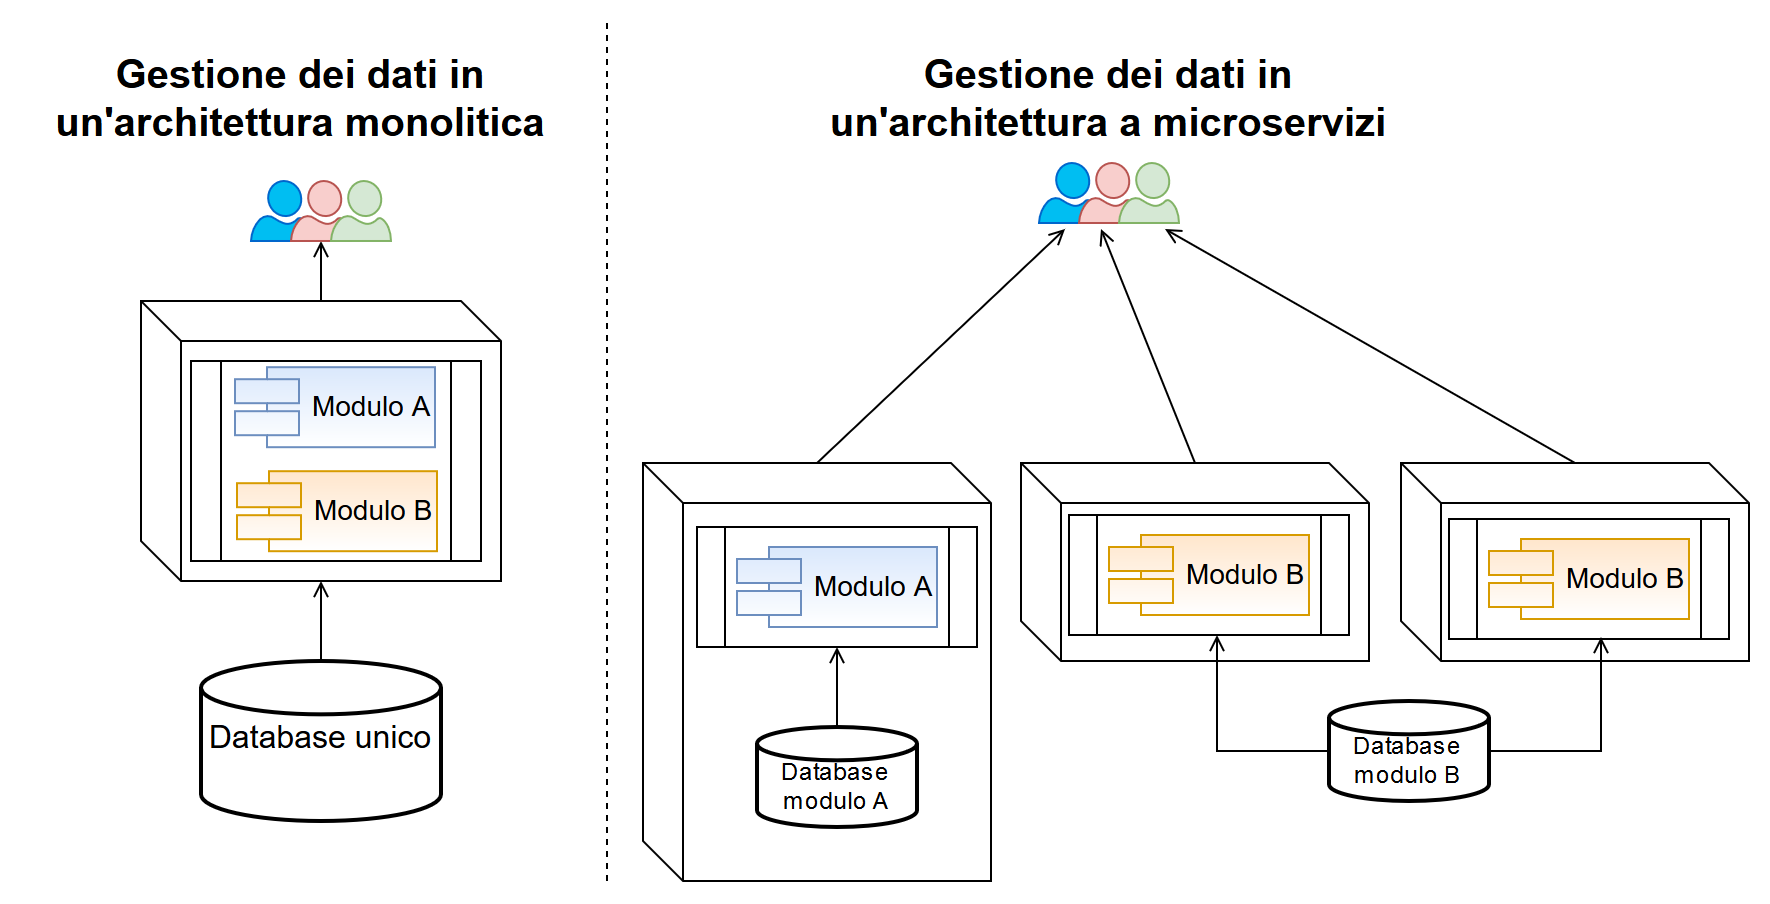
\includegraphics[width=0.9\columnwidth]{intro/data-storage}
    \caption{Illustrazione che mostra la differente gestione dell'architettura di persistenza dei dati tra prodotti software con architettura monolitica e con architettura a microservizi.}
    \label{fig:data-storage}
\end{figure}

La decentralizzazione delle decisioni di \emph{storage} implica una maggior attenzione verso gli aggiornamenti dei dati.
L'approccio comune agli aggiornamenti in un'architettura monolitica è quello di usare le transazioni per garantire la consistenza dei dati prima e dopo ciascun aggiornamento.
L'utilizzo di transazioni è un grave limite per l'architettura a microservizi, in quanto le transazioni impongono un ordine temporale che potrebbe non essere rispettato, causando inconsistenze dei dati salvati.
É per questo che le architetture a microservizi enfatizzano l'utilizzo di comunicazioni non vincolanti (transactionless): eventuali inconsistenze vengono segnalate e risolte grazie a operazioni correttive.

Una conseguenza nell'utilizzo dei servizi come componenti è che le applicazioni devono prevedere e tollerare malfunzionamenti nei servizi. L'utilizzatore dei servizi deve quindi rispondere ai malfunzionamenti nel modo più elegante possibile. Dato l'aumento di complessità, questo è da annoverare tra i difetti delle architetture a microservizi. Dal momento che i servizi possono malfungere in ogni momento, è fondamentale riuscire a:

monitorare il servizio,
segnalare il malfunzionamento e
ripristinare automaticamente il servizio
nel più breve tempo possibile. Conseguentemente, ogni servizio deve essere progettato focalizzando l'attenzione sulle attività di monitoring, individuando le metriche rilevanti (ad es. throughput, latenza, ecc.).

Utilizzando i servizi come componenti ci si chiede spesso quante responsabilità debba avere ciascun servizio: la caratteristica fondamentale da osservare è la nozione di sostituzione e aggiornamento indipendenti.
Un buon segnale lo si ritrova quando ad ogni modifica di un servizio, questa modifica non richiede adattamenti in altri servizi (a meno di modifiche di funzionalità offerte).
Se 2 o più servizi vengono aggiornati spesso insieme probabilmente essi dovrebbero essere uniti.

%**************************************************************
\section{Rischi}

I rischi collegati allo svolgimento di questo stage possono essere suddivisi in tre categorie:
\begin{itemize}
  \item rischi collegati alla scelta dello stage nella sua forma interna;
  \item rischi collegati alla scelta del tema IoT;
  \item rischi collegati alla scelta dell'architettura a microservizi.
\end{itemize}


\subsection{Rischi: Stage interno}

Lo stage formativo viene previsto dal CdL triennale di Informatica in due modalità:
\begin{itemize}
  \item stage aziendali, riferiti anche come stage esterni, per i quali il proponente del progetto di stage è un'azienda;
  \item stage non aziendali, riferiti anche come stage interni, per i quali il proponente del progetto di stage è un docente dell'Ateneo di Padova.
\end{itemize}


Sebbene lo stage aziendale sia la modalità preferita per svolgere l'attività, mi sono imbattuto in un ostacolo che mi ha portato ad avviare uno stage interno.
Dato il periodo di inizio dello stage (ottobre/novembre 2017), molti degli stage aziendali proposti sono stati soddisfatti da altri studenti del corso.
Le aziende contattate non avevano pianificate attività di stage nell'ambito dell'IoT per il \emph{timeframe} richiesto: pensando alle premesse esposte in \hyperref{intro-iot}, ho scelto di iniziare a valutare il percorso di stage non aziendale.

In uno stage non aziendale i rischi considerati sono elencati nella tabella ~\ref{tab:rischi-stage-interno}.

\begin{table}
\caption{Tabella di analisi dei rischi correlati allo svolgimento di uno stage interno}
\label{tab:rischi-stage-interno}
\begin{tabularx}{\linewidth}{|p{7.5cm}|X|X|}
\hline
\textbf{Rischio} & \textbf{Probabilità di accadimento} & \textbf{Gravità del danno potenziale}\\
\hline
Il lavoro svolto individualmente, senza possibilità di essere guidato da esperti nel settore, potrebbe risultare ininfluente. La presenza di una persona con più esperienza in un determinato tema è utile in quanto può focalizzare l'attenzione su problematiche reali, le quali potrebbero non essere correttamente valutate nel momento in cui si dispone di scarsa esperienza in materia. & Molto probabile & Grave \\
\hline
Il lavoro svolto individualmente, senza possibilità di essere guidato da esperti nel settore, potrebbe procedere più lentamente, causando il non raggiungimento degli obiettivi preposti. & Molto probabile & Media \\
\hline
\end{tabularx}
\end{table}


\subsection{Rischi: IoT}

https://medium.com/@Imaginovation/iot-security-risks-and-benefits-18428819e735

A causa della relativa novità dell'argomento, il settore IoT si pone a numerose osservazioni relative ai rischi collegati allo sviluppo di prodotti software e hardware. I rischi considerati sono elencati nella tabella ~\ref{tab:rischi-iot}.
\begin{table}
\caption{Tabella di analisi dei rischi correlati al tema IoT}
\label{tab:rischi-iot}
\begin{tabularx}{\linewidth}{|p{7.5cm}|X|X|}
\hline
\textbf{Rischio} & \textbf{Probabilità di accadimento} & \textbf{Gravità del danno potenziale}\\
\hline
Lo sviluppo di prodotti legati all'IoT espone l'utente degli stessi a possibili rischi di cybersicurezza: il furto di dati ma soprattutto la perdita di controllo dell'utente sui propri dispositivi sono scenari possibili e con conseguenze disastrose per lo sviluppatore di tale prodotto. & Probabile & Molto grave \\
\hline
La mole di dati raccolta dai dispositivi inseriti in un contesto IoT potrebbe essere tale da richiedere investimenti consistenti per la loro elaborazione e per mantenere elevata la loro confidenzialità. Inoltre la diversità dei dispositivi presenti in una rete aumenta la complessità del trattamento delle informazioni. & Probabile & Media \\
\hline
Dal momento che l'IoT è un ambito emergente nel contesto ITC è possibile osservare la nascita di una multitudine di protocolli per la raccolta e la trasmissione delle informazioni, nessuno dei quali è stato indicato come standard globale. & Molto probabile & Media \\
\hline
\end{tabularx}
\end{table}


\subsection{Rischi: Architettura a microservizi}



Illustrare i rischi derivati dalle scelte effettuate.

%**************************************************************
\section{Struttura del documento}

Il presente documento prosegue nei seguenti 3 capitoli
\begin{description}
    \item[{\hyperref[cap:processi-metodologie]{Il secondo capitolo}}] descrive con maggior precisione il progetto di stage, elencandone gli obiettivi curricolari, formativi, tecnici e di prodotto.

    \item[{\hyperref[cap:descrizione-stage]{Il terzo capitolo}}] approfondisce il lavoro svolto durante lo svolgimento dello stage, esaminando le attività di analisi, progettazione, codifica e test.

    \item[{\hyperref[cap:analisi-requisiti]{Il quarto capitolo}}] fornisce una valutazione degli obiettivi raggiunti, motivando la presenza di eventuali obiettivi non raggiunti; inoltre vengono esaminate le conoscenze acquisite e i rischi descritti nel presente capitolo.

    % \item[{\hyperref[cap:progettazione-codifica]{Il quinto capitolo}}] approfondisce ...
    %
    % \item[{\hyperref[cap:verifica-validazione]{Il sesto capitolo}}] approfondisce ...
    %
    % \item[{\hyperref[cap:conclusioni]{Nel settimo capitolo}}] descrive ...
\end{description}

\section{Convenzioni tipografiche}

Riguardo la stesura del testo, relativamente al documento sono state adottate le seguenti convenzioni tipografiche:
\begin{itemize}
	\item gli acronimi, le abbreviazioni e i termini ambigui o di uso non comune menzionati vengono definiti nel glossario, situato alla fine del presente documento;
	\item per la prima occorrenza dei termini riportati nel glossario viene utilizzata la seguente nomenclatura: \emph{parola}\glsfirstoccur;
	\item i termini in lingua straniera o facenti parti del gergo tecnico sono evidenziati con il carattere \emph{corsivo}.
\end{itemize}
